% !TEX program = xelatex
% vim:foldmethod=marker:foldmarker=<<<,>>>
\documentclass[compress,aspectratio=169]{beamer}

%<<< Preamble
\usepackage[english]{babel}
\usepackage{metalogo}
\usepackage{listings}
\usepackage{fontspec}
\usepackage{amsmath, amssymb, bm}
\usepackage{stackrel}
\usepackage{tikz}
\usepackage{unicode-math}
\usepackage{subcaption}
\usepackage[theme=nord,charsperline=60,linenumbers]{jlcode}
% \usepackage[charsperline=60,linenumbers]{jlcode}

% \usetheme{Boadilla}
\usetheme{Nord}

\setmainfont{Roboto}
% \setsansfont{DejaVu Serif}
% \setmonofont{CaskaydiaCove Nerd Font Mono}
\setmonofont{JuliaMono}

\setbeamercolor{mybullet}{use=itemize item.fg,bg=itemize item.fg,fg=itemize item.fg}

\makeatletter
\def\verbatim@nolig@list{}
\newcommand\pin{%
\parbox[t]{10pt}{\raisebox{0.2pt}{\usebeamercolor[fg]{mybullet}{$\ast$}}}}
\makeatother

\newcommand{\E}[1]{\ensuremath{E\left\{#1\right\}}}
\newcommand{\norm}[1]{\ensuremath{\lVert#1\rVert}}
\newcommand*{\thead}[1]{\multicolumn{1}{c}{\fseries #1}}

\newfontfamily\tabulartext[SizeFeatures={Size=6}]{Roboto}

\hypersetup{
    colorlinks=true,
    urlcolor=NordBlue
}

\DeclareMathOperator*{\argmax}{argmax}
\DeclareMathOperator*{\Var}{Var}
\DeclareMathOperator*{\test}{\gtrless}

\AtBeginDocument{
    \fontsize{8}{12}
    \selectfont

}

\AtBeginSection[]
{
    \begin{frame}[c,noframenumbering,plain]
        \tableofcontents[sectionstyle=show/hide,subsectionstyle=show/show/hide]
    \end{frame}
}


\AtBeginSubsection[]
{
    \begin{frame}[c,noframenumbering,plain]
        \tableofcontents[sectionstyle=show/hide,subsectionstyle=show/shaded/hide]
    \end{frame}
}
%>>>

\title{Project V: Signal Modelling}
\subtitle{}
\author{\large Simon Andreas Bjørn}
\date{\large March 14, 2023}

\begin{document}

\begin{frame}[plain,noframenumbering]
    \maketitle
\end{frame}

\begin{frame}[fragile] % <<< Functions for linear prediction
    \frametitle{Functions for linear prediction}
    We start by implementing the 2 possible methods for linear prediction.

    \begin{columns}
        \begin{column}{0.5\textwidth}

            Implemented by folloing lecture notes
            \begin{jllisting}[gobble=16]
                 function corrpred(x, p, r)
                    N = length(x)
                    X = zeros(N+p, p)
                    for i=1:p
                        X[i:i+N-1,i] = x
                    end

                    b = [zeros(p);x]
                    a = [1; vec(reverse(-X \ b))]
                    err = mean((x - filt(1.0, a, [1; zeros(N-1)])).^2)
                    return [a, err]
                end
            \end{jllisting}
        \end{column}
        \begin{column}{0.5\textwidth}

            Implemented by following the book
            \begin{jllisting}[gobble=16]
                function covpred(x, p, r)
                    N = length(x)
                    X = zeros(N+p, p)
                    for i=1:p
                        X[i:i+N-1,i] = x
                    end
                    X = X[p:N-1,:] 
                    b = x[p+1:N]
                    a = [ 1; -X \ b ]
                    err = mean((x - filt(1.0, a, [1; zeros(N-1)])).^2)
                    return [a, err]
                end
            \end{jllisting}
        \end{column}
    \end{columns}
    
    Testing both function on the filter \jlinl{b=1.0, a=[1.0, 0.2, 0.3]}, I get
    \begin{jllisting}[gobble=8]
        x = filt(1.0, [1,0.2,0.3], [1; zeros(100)])
        @show corrpred(x, 2, 0); # -> corrpred(x, 2, 0) = Any[[1.0, 0.2, 0.3], 4.523e-35]
        @show covpred(x, 2, 0);  # -> covpred(x, 2, 0)  = Any[[1.0, 0.2, 0.3], 5.611e-35]
    \end{jllisting}

\end{frame} 
% >>>

\begin{frame}[fragile] % <<< Testing code on ARdata
    \frametitle{Testing code on ARdata}
    We now want to test our code on the provided \jlinl{ARdata.mat} file.
    \begin{jllisting}[gobble=8]
        @show a1 # -> a1 = [1.0, -1.9099, 1.3989, -0.4949]
        @show corrpred(x1, 3, 0); # -> corrpred(x1, 3, 0) = Any[[1.0, -1.1126, 0.1291, 0.0061], 21.1632]
        @show covpred(x1, 3, 0); # -> covpred(x1, 3, 0) = Any[[1.0, -1.9099, 1.3989, -0.4948], 8.8982]
    \end{jllisting}
    \begin{columns}
        \begin{column}{0.53\textwidth}
            Then we want to plot a pole-zero plot of the  true coefficients. No
            in-built pole-zero plot, so define a simple plot function.
            \begin{jllisting}[gobble=16]
                function zplane!(ax::Axis, sys::LTISystem)
                    z = tzeros(sys)
                    p = poles(sys)
                    return [
                        scatter!(ax, real(z), imag(z), marker='o'),
                        scatter!(ax, real(p), imag(p), marker='x')
                    ]
                end
            \end{jllisting}
        \end{column}
        \begin{column}{0.47\textwidth}
            \begin{figure}
                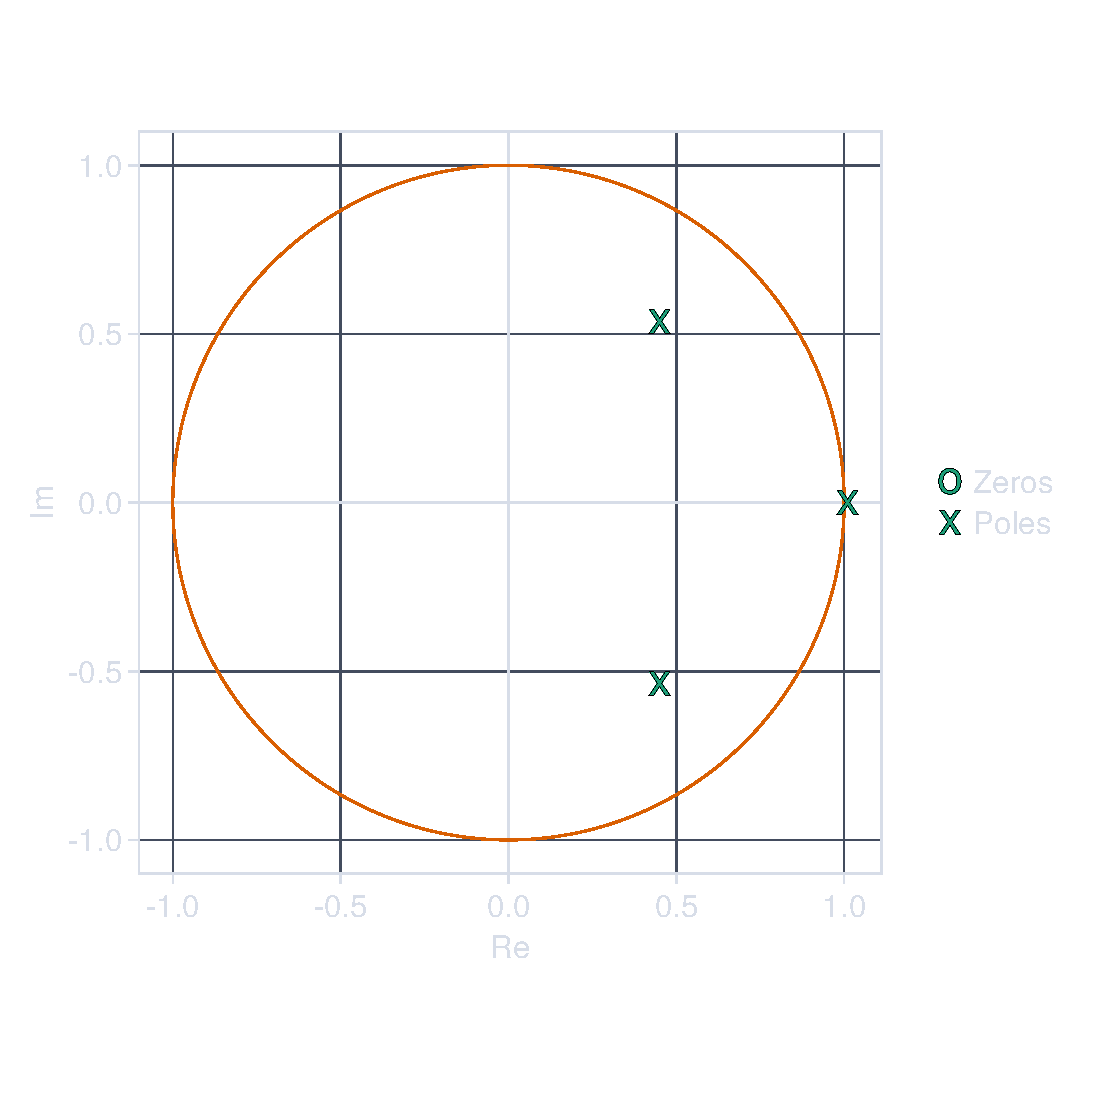
\includegraphics[width=0.8\columnwidth]{"../1.pdf"}
            \end{figure}
        \end{column}
    \end{columns}
    
\end{frame}
% >>>

\begin{frame}[fragile] % <<< Pole-zero plot of coefficients from methods
    \frametitle{Pole-zero plot of coefficients from methods}

    Now we want to plot the coefficients we get from predicting the coefficients.
    Estimating the coefficients, I create a transferfunction per method and
    plot the resulting LTISystem using \jlinl{zplane()} function.
    \begin{jllisting}[gobble=8]
        a1_corr, err1_corr = corrpred(x1, 3, 1)
        a1_cov, err1_cov   = covpred(x1, 3, 1)
        zplane!(ax1, tf([1.0], a1)); zplane!(ax2, tf([1.0], a1_corr)); zplane!(ax3, tf([1.0], a1_cov))
    \end{jllisting}
    and get the following plots
    \begin{figure}
        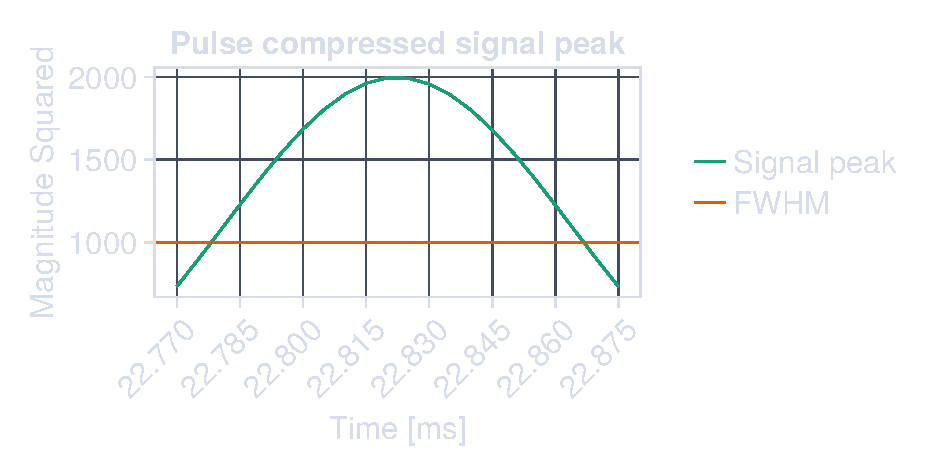
\includegraphics[width=0.8\columnwidth]{"../2.pdf"}
    \end{figure}
\end{frame}
% >>>

\begin{frame} % <<< Pole-zero plot of x2
    \frametitle{Pole-zero plot of x2}
    Now we do the same but predicting on the x2 sequence.
    
    \begin{figure}
        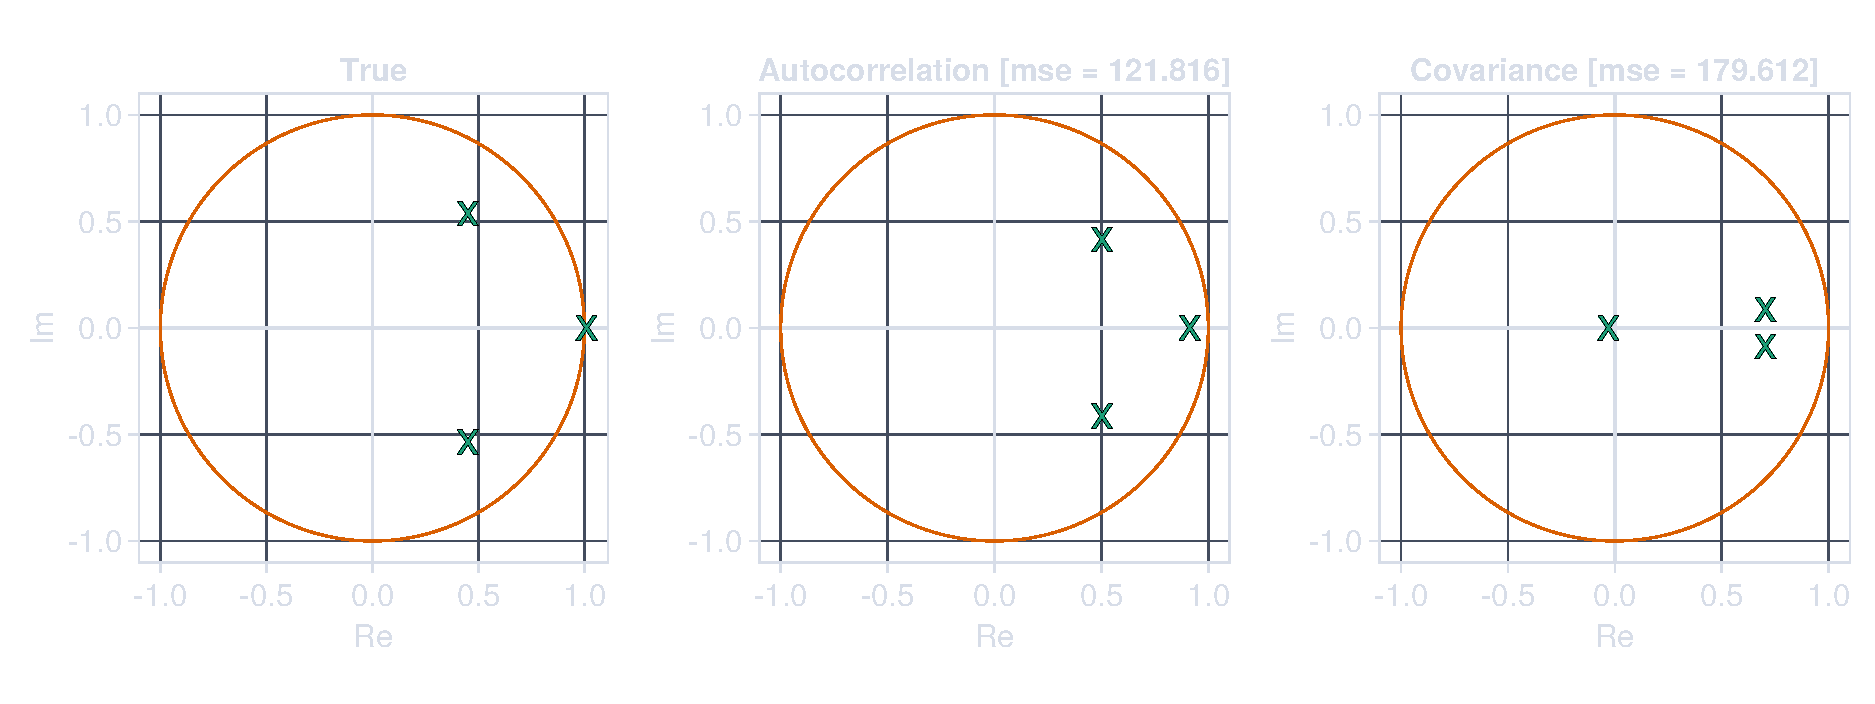
\includegraphics[width=\columnwidth]{"../3.pdf"}
    \end{figure}
\end{frame} % >>>

\begin{frame} % <<< Iterating order and estimating x3
    \frametitle{Iterating order and estimating x3}
    We want to loop over the filter order and estimate the filter coefficients for
    x3.
    Plotting the MSE of each method per iteration, I have
    \begin{figure}
        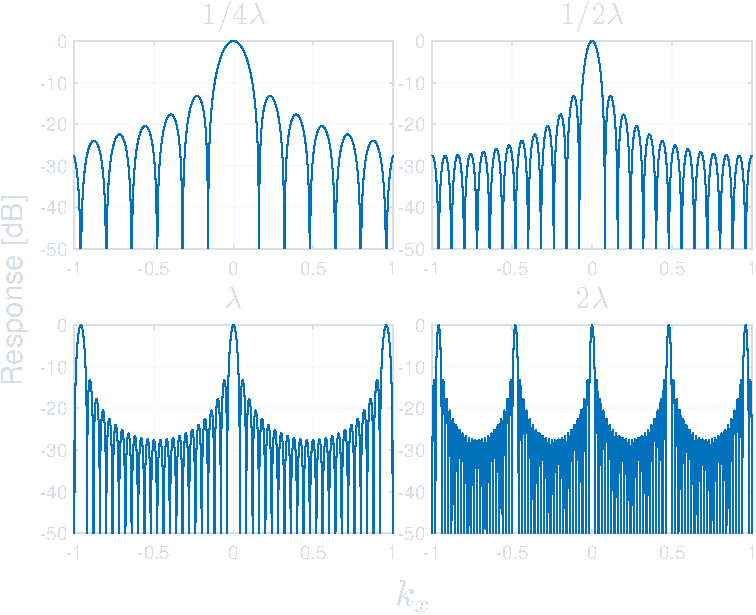
\includegraphics[width=0.6\columnwidth]{"../4.pdf"}
    \end{figure}
    \begin{itemize}
        \item Covariance is a bit strange after order $P=4$. Should flatten out.
        \item MSE is within the same order of magnitude between the methods
        \item Using the solution provided in the assignment, I conclude with P=4
            as a good estimate of the filter order.
        \item Flattening out means no more dimensions can improve the estimate.
    \end{itemize}
\end{frame}
% >>>

\begin{frame}[fragile] % <<< Frequency response of new filter
    \frametitle{Frequency response of new filter}
    Now we have a new filter with \jlinl{b = 5; a = [1, -1.3, 0.845]}. Now we
    want to plot the true power spectrum.

    \begin{jllisting}[gobble=8]
        x = [1; zeros(N-1)]; h = filt(b, a, x)
        H_true = fftshift(fft(h))[end÷2:end];
        P_h_true = abs.(H_true.^2); P_h_true /= length(P_h_true)
    \end{jllisting}

    Plotting the true power spectrum and the phase angle, I get the following
    plots.

    \begin{columns}
        \begin{column}{0.45\textwidth}
            \begin{figure}
                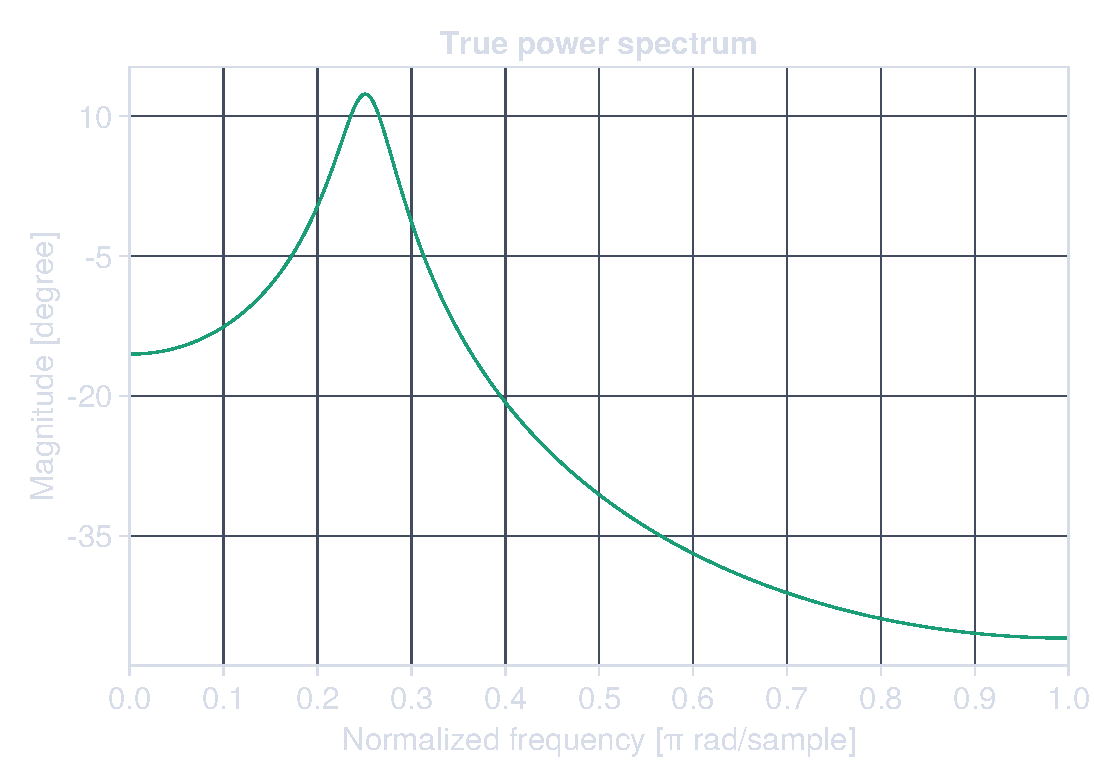
\includegraphics[width=\columnwidth]{"../5.pdf"}
            \end{figure}
        \end{column}
        \begin{column}{0.55\textwidth}
            \begin{figure}
                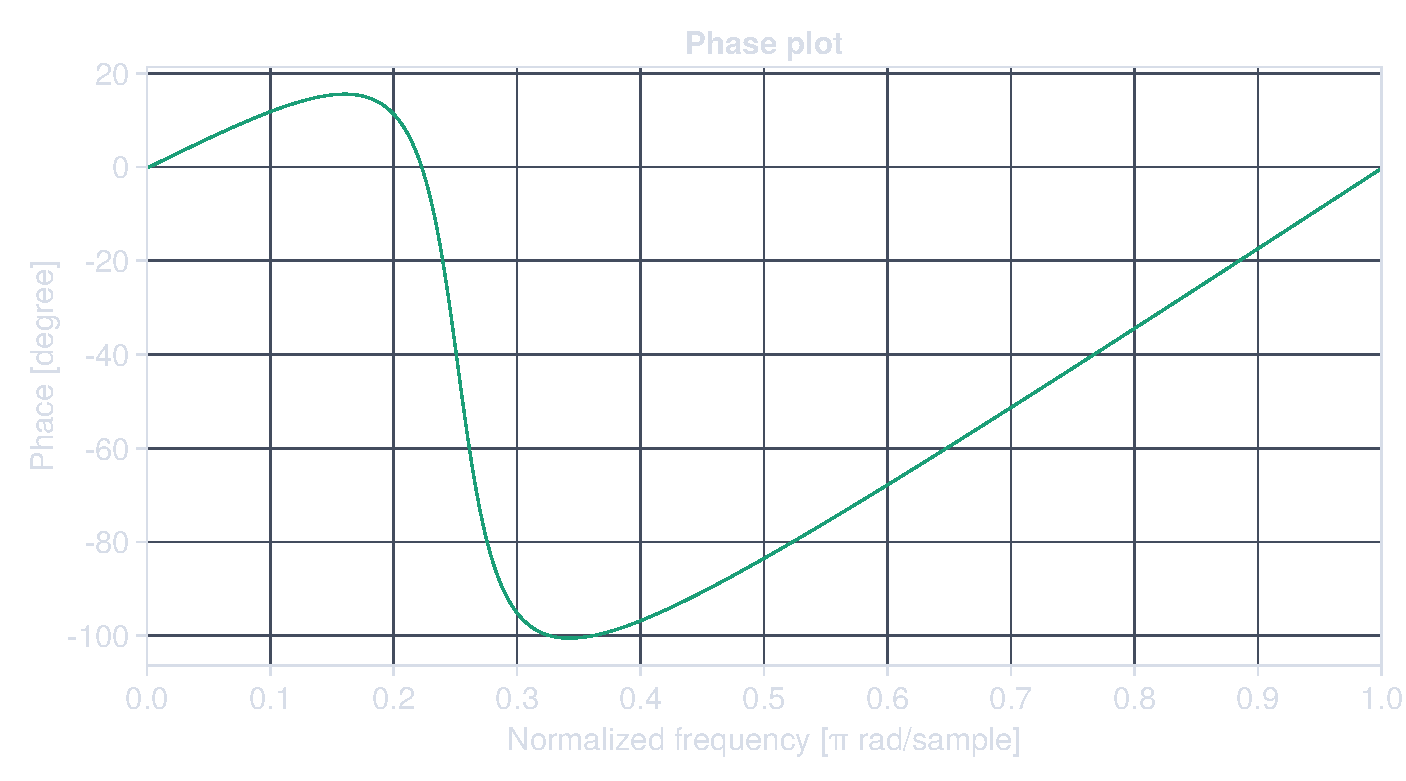
\includegraphics[width=\columnwidth]{"../6.pdf"}
            \end{figure}
        \end{column}
    \end{columns}
\end{frame}
% >>>

\begin{frame} % <<< Noise driven filten experiment
    \frametitle{Noise driven filten experiment}
    Now we want to estimate the coefficients of the filter using random noise.
    Instead of using the impuls response, we use gaussian white noise.
    Estimating this and plotting similarly to the previous plots, I get
    \begin{figure}
        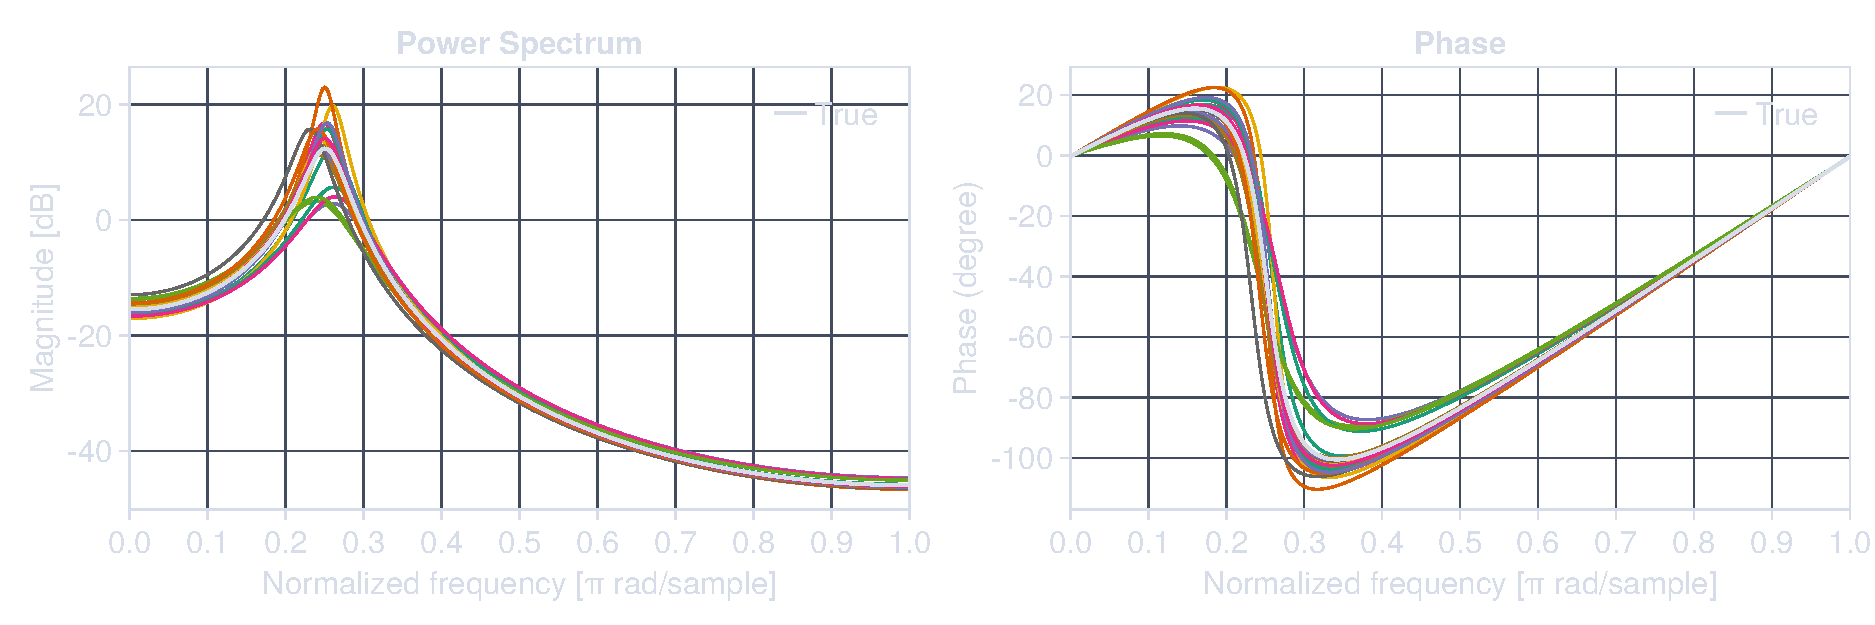
\includegraphics[width=\columnwidth]{"../7.pdf"}
    \end{figure}
\end{frame} % >>>

\begin{frame} % <<< Pole-zero plot from noise
    \frametitle{Pole-zero plot from noise}
    Now, using the coefficients found in the previous task, we plot a pole-zero
    plot.
    \begin{columns}
        \begin{column}{0.5\textwidth}
            \begin{itemize}
                \item Small scattering a round true poles
            \end{itemize}
        \end{column}
        \begin{column}{0.5\textwidth}
            \begin{figure}
                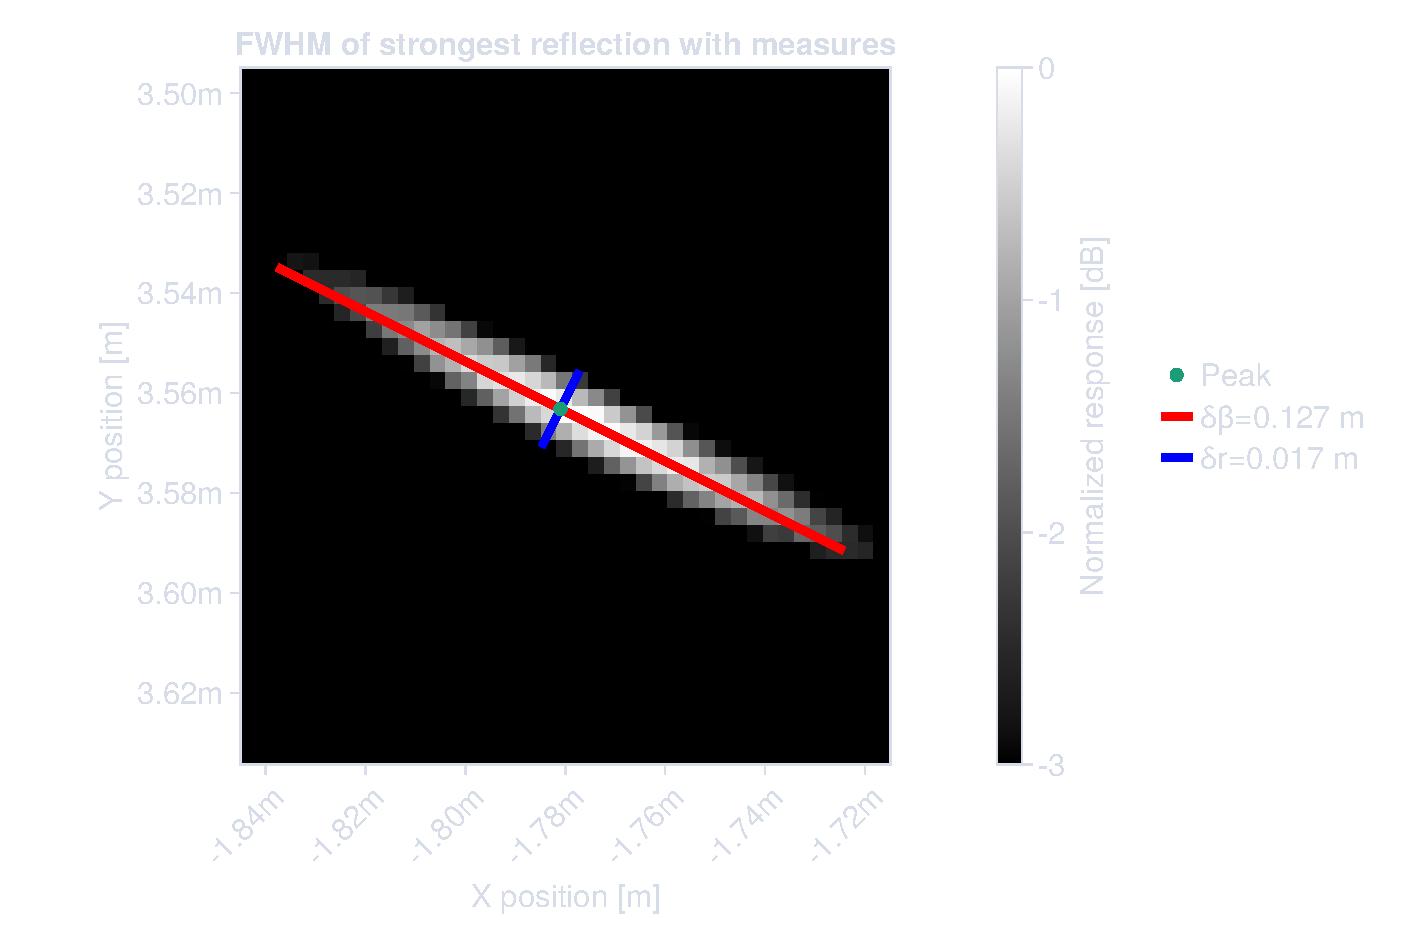
\includegraphics[width=\columnwidth]{"../8.pdf"}
            \end{figure}
        \end{column}
    \end{columns}
\end{frame} % >>>

\begin{frame}[fragile] % <<< Testing with longer sequences
    \frametitle{Testing with longer sequences}
    Now we increase the number of samples we use to estimate.
    Code is then
    \begin{jllisting}[gobble=8]
        x = randn(N)
        h = filt(b, a, x)
        h_samples = h[20:20+1000]
        h_samples2 = h[20:20+10_000]
    \end{jllisting}
    Plotting this I get
    \begin{figure}
        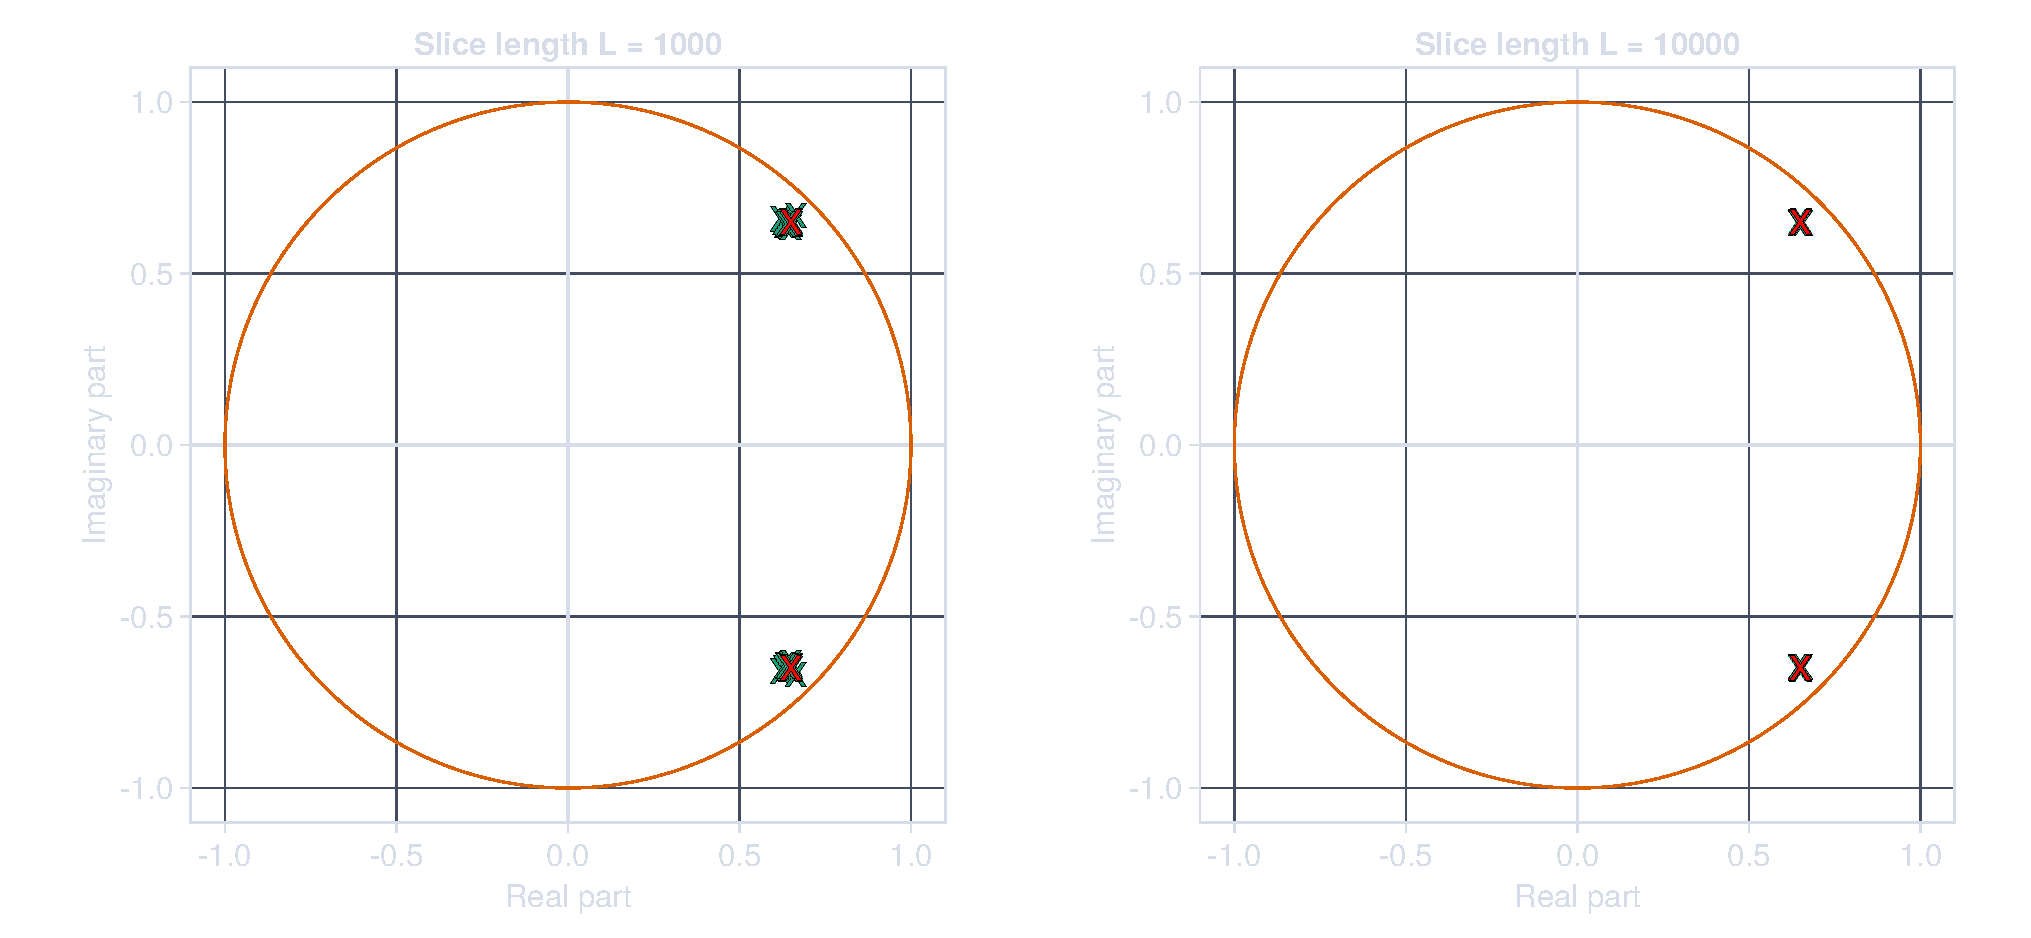
\includegraphics[width=0.7\columnwidth]{"../9.pdf"}
    \end{figure}

\end{frame}
% >>>

\begin{frame}[fragile] % <<< Tapering the sequence
    \frametitle{Tapering the sequence}
    Very lastly, we want to try and taper the x-sequences with a Hamming window,
    and compare them to using unit weights (boxcar).
    Code is then
    \begin{jllisting}[gobble=8]
        h1 = filt(b, a, x)
        h2 = filt(b, a, x.*hamming(N))
    \end{jllisting}

    Plotting them to compare with both $L=128$ and $L=256$, I get the following
    plots
    \begin{figure}
        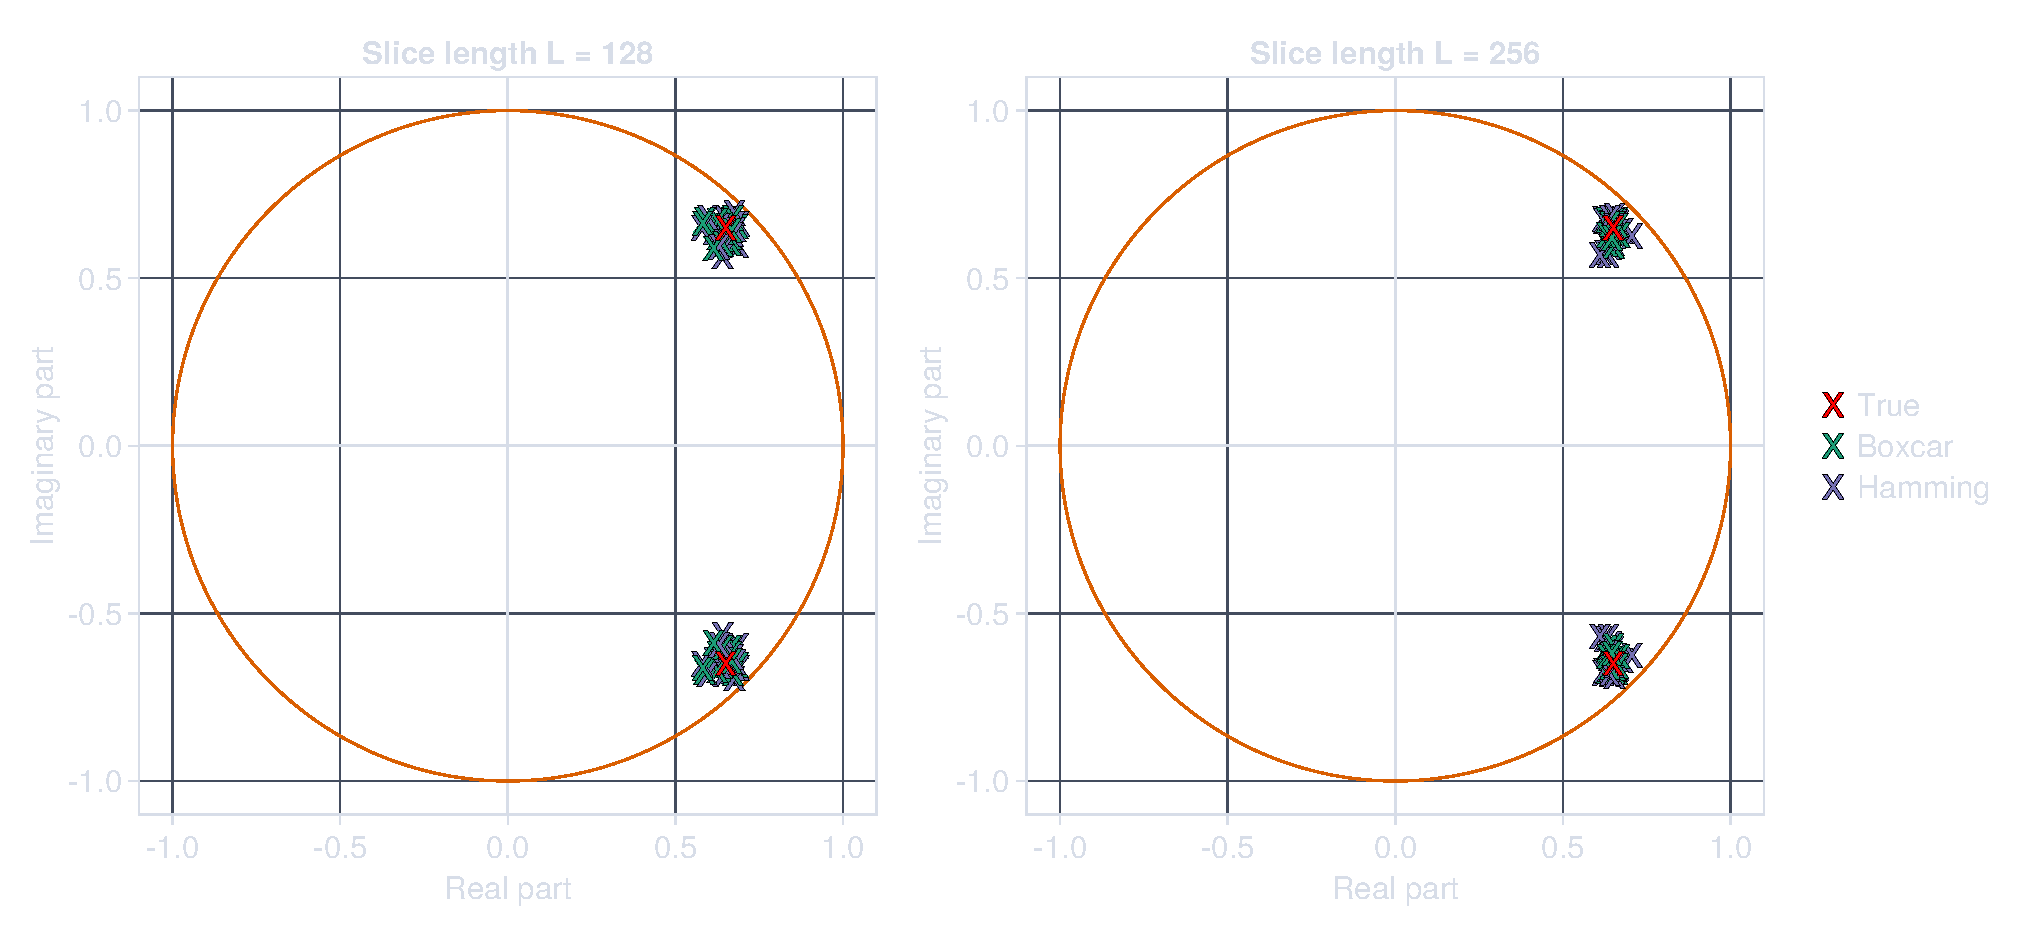
\includegraphics[width=0.65\columnwidth]{"../10.pdf"}
    \end{figure}
\end{frame}
% >>>

\end{document}
